\title{Concurrency and Parallel Programming \\ Assignment 1}
\author{David van Erkelens and Jelte Fennema \\ Department of Computer Science
    \\ University of Amsterdam} \date{\today}
\documentclass[12pt]{article}
\usepackage{graphicx}
\usepackage{color}
\begin{document}
\maketitle
\section{Assignment 1.1}

As can be seen in the graph, the speedup differs a lot between the different
problem sizes. With the smallest problem size, i\_max = $10^3$, the speedup
with all amount of threads is lower than one. This means that using the
sequential algorithm  is the fastest is this specific case. This is probably
caused by the relatively high amount of time that is spent in the critical
section with small problem sizes. With i\_max = $10^4$ the maximum speedup is at
two threads. After that it goes downhill quickly. \\
The three largest problem sizes all benefit from more threads. The most likely
reason for this is that waiting in a critical section occurs less per
calculations a thread does.\ i\_max = $10^6$ has the largest speedup. With eight
threads it reaches a speedup of a little above five.

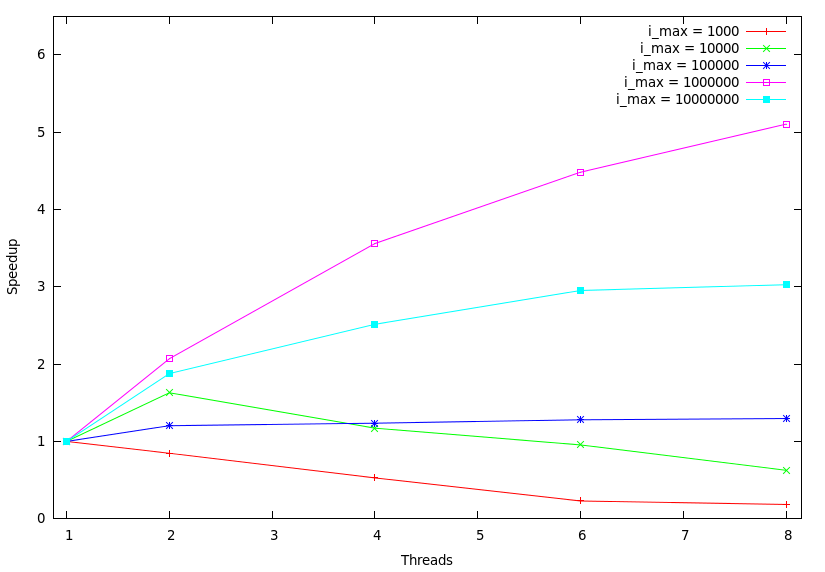
\includegraphics[width=\textwidth]{speedupgraph.png}

\section{Assignment 1.2}
This is where I, David, will add my findings regarding assignment 1.2.
\end {document}
